%; whizzy chapter
% -initex iniptex -latex platex -format platex -bibtex jbibtex -fmt fmt
% 以上 whizzytex を使用する場合の設定。


%     Tokyo Debian Meeting resources
%     Copyright (C) 2008 Junichi Uekawa

%     This program is free software; you can redistribute it and/or modify
%     it under the terms of the GNU General Public License as published by
%     the Free Software Foundation; either version 2 of the License, or
%     (at your option) any later version.

%     This program is distributed in the hope that it will be useful,
%     but WITHOUT ANY WARRANTY; without even the implied warranty of
%     MERCHANTABILITY or FITNESS FOR A PARTICULAR PURPOSE.  See the
%     GNU General Public License for more details.

%     You should have received a copy of the GNU General Public License
%     along with this program; if not, write to the Free Software
%     Foundation, Inc., 51 Franklin St, Fifth Floor, Boston, MA  02110-1301 USA

%  preview (shell-command (concat "evince " (replace-regexp-in-string "tex$" "pdf"(buffer-file-name)) "&"))
% 画像ファイルを処理するためにはebbを利用してboundingboxを作成。
%(shell-command "cd image200801; ebb *.png")

%%ここからヘッダ開始。

\documentclass[mingoth,a4paper]{jsarticle}
\usepackage{monthlyreport}

% 日付を定義する、毎月変わります。
\newcommand{\debmtgyear}{2008}
\newcommand{\debmtgmonth}{3}
\newcommand{\debmtgdate}{15}
\newcommand{\debmtgnumber}{38}

\begin{document}

\begin{titlepage}
\thispagestyle{empty}

% タイトルページ:編集必要な部分は最初のマクロに飛ばすこと

\vspace*{-2cm}
第\debmtgnumber{}回 東京エリア Debian 勉強会資料

\hspace*{-2.4cm}
\includegraphics[width=210mm]{image200801/2008title.eps}\\
\hfill{}\debmtgyear{}年\debmtgmonth{}月\debmtgdate{}日

\end{titlepage}

\dancersection{Introduction}{上川 純一}
 
 今月のDebian勉強会へようこそ。これからDebianの世界にあしを踏み入れると
 いう方も、すでにどっぷりとつかっているという方も、月に一回Debianについ
 て語りませんか?

 Debian勉強会の目的は下記です。

\begin{itemize}
 \item \underline{Debian Developer} (開発者)の育成。
 \item 日本語での「\underline{開発に関する情報}」を整理してまとめ、アップデートする。
 \item \underline{場}の提供。
 \begin{itemize}
  \item 普段ばらばらな場所にいる人々が face-to-face で出会える場を提供
	する。
  \item Debian のためになることを語る場を提供する。
  \item Debianについて語る場を提供する。
 \end{itemize}
\end{itemize}		

 Debianの勉強会ということで究極的には参加者全員がDebian Packageをがりがり
 と作るスーパーハッカーになった姿を妄想しています。情報の共有・活用を通し
 て Debianの今後の能動的な展開への土台として、「場」としての空間を提供す
 るのが目的です。

以上を目的とした、2008 年アジェンダです:
\begin{enumerate}
 \item 新年会「気合を入れる」
 \item Open Source Conference Tokyo (3/1)
 \item データだけのパッケージを作成してみる、
       ライセンスの考え方 (David Smith)
 \item バイナリ一つのパッケージを作成してみる (吉田@板橋)\\
       バージョン管理ツールを使いDebianパッケージを管理する(git)\\
       アップストリームの扱い(svn/git/cvs)(岩松 信洋さん)
 \item バイナリの分けたパッケージの作成。(前田さん)\\
       バイナリの分け方の考え方、アップグレードなどの運用とか。
 \item パッケージ作成(dpatch/debhelperで作成するパッケージ)(小林儀匡さん)\\
       man の書き方(roff or docbook)(でんさん)
 \item パッケージ作成(kernel patch、kernel module)
       、Debconf発表練習
 \item Debconf アルゼンチン、共有ライブラリパッケージ作成

 \item Open Source Conference Tokyo/Fall、
       デーモン系のパッケージの作成、latex、 emacs-lisp、フォントパッケージ
 \item パッケージの cross-compile の方法、amd64 上で i386 のパッケージと
       か、OSC-Fall報告会、Debconf報告会
 \item 国際化 po-debconf / po化 / DDTP
 \item 忘年会
\end{enumerate}


\newpage

\begin{minipage}[b]{0.2\hsize}
 \definecolor{titleback}{gray}{0.9}
 \colorbox{titleback}{\rotatebox{90}{\fontsize{80}{80} {\gt デビアン勉強会} }}
\end{minipage}
\begin{minipage}[b]{0.8\hsize}
\hrule
\vspace{2mm}
\hrule
\setcounter{tocdepth}{1}
\tableofcontents
\vspace{2mm}
\hrule
\end{minipage}

%===========================================================%
\dancersection{事前課題}{上川 純一}
%===========================================================%

今回の事前課題は以下から自由に選択して200-800文字で回答するというものでした。

\begin{enumerate}
 \item データだけのパッケージでできること
 \item ソフトウェアのライセンスで不自由したこと
 \item 好きなソフトウェアライセンスとその理由
\end{enumerate}

この課題に対して提出いただいた内容は以下です。

\begin{multicols}{2}
{\footnotesize
\subsection{堀内寛己}

僕が好きなソフトウェアライセンスはGPLです。
理由は、ストールマンが好きだからです。

僕がストールマンのことを知ったのは、
20年以上前、東大の和田英一先生の講義をもぐって聞いたときのことです。
先生は、MITハッカーズの堕落と、
その中で孤軍奮闘しているストールマンの話をされました。
「でもストールマンは変わりませんねえ。
グニューって知ってますか? みんなタダなんですよ」
先生が英語の微妙なニュアンスを聞き分けられないわけがないので、
当時のストールマン自身が、freeの2つの意味を混同していたらしいことがわかります。
当然そのころ、GPLなんてありませんでした。
僕は幸い、入社まもなくGNU Emacsを使う幸運に恵まれ、
ストールマンへの敬意は確固たるものになり、
そのままGPLのことなど知らずにgcc-2のmakeをやったものです。
僕がGPLとその恐るべき意図について知ったのは、だいぶ後のことです。
Microsoftがこれをウィルス呼ばわりしたのほ、さらにその後のことです。
僕は、ウィルスという表現は、GPLについての最高の褒め言葉だと思っています。


\subsection{山本ひろゆき}

「データだけのパッケージでできること」
インタープリタ依存のスクリプトパッケージなんかができますかね?今抱えてい
る ITP を片付けたら、kita2 (ruby スクリプト) を ITP しようかと迷っていま
す。パッケージング自体はできますが、ruby を知らないものでメンテナンスが
心配。誰か教えて!

「ソフトウェアのライセンスで不自由したこと」
某巨大掲示板発祥の開発プロジェクトあたりだと、有用なソフトウェアだが、ラ
イセンスは明記されていなく開発者も匿名で確認しようがないということもあり
ます。

「好きなソフトウェアライセンスとその理由」
GPL とか BSD ライセンスとか。DFSG 万歳!



\subsection{Suguru Sekine}
「好きなソフトウェアライセンスとその理由」

[BSDライセンス]

 自由であり続けるために「自由でなければならない」という制約がない、
かつソースコードの公開を拒む自由があるためである。
私はソフトウェアは自由であるべきだと考えている。
また、自由であるための協力もできる限りの協力を行うつもりである。
しかし、自分が考えている事を他の人に強要したり、
または強要されたりすることがどうしても我慢できない。
以上のことから自由であることを強要されない点から
BSDライセンスをを評価しているという結論に至る。

\subsection{Yamane Toshiaki}

「データだけのパッケージでできること」

データだけのパッケージというものが例えばフォントパケジ等を
指すという理解で文章を書いてみます。
できること、ではないかもしれませんが、自分が使いたいものを
選択する自由があると考えます。あるいは X と xfont なパッケージのように
アプリケーションとデータがそれぞれ互いに依存していない関係にする事が
できるのではないか、と考えます。データだけのパッケージと
そのデータを使うパッケージ間を疎結合な関係にしておくことによって、
保守とか拡張などの対応を柔軟に行なう事ができるのではないでしょうか。

\subsection{沖中}

ライセンス的に配布が難しいデータは、自分でパッケージすることになると思いますが、
データだけのパッケージと言えばフォントが代表的だと思います。
辞書データもフリーの物が少ないので自分でパッケージ化できたら便利ですね。
それ以外の使い方としては、Webサイトのドキュメントをパッケージ化して
管理できないか考えています。そうなるとデータだけとはいきませんが、スクリプトだと
ビルド不要なのでデータと同じように扱えるのではと思ってます。


\subsection{山根秀樹}

ソフトウェアのライセンスで不自由したこと

 今まさに不自由してます。いわゆる「フリーフォント」が巷にはたくさんあるのですが、
 みんな「自分で規定しましたライセンス」が多くて、二次利用などがしづらいですね。
 作者の方々は善意で策定したんでしょうけど、「悪いことに使っちゃダメ」ライセンス
 みたいなのは勘弁して欲しいです(線引きが曖昧だし、そもそも悪いことしようとする
 人がライセンスを気にすることなんぞ無いわけで、そんな規定作ること自体が意味ない
 んですが…)。

 あとは最近あったのが PHP プロダクトで PHP ライセンスのものとか。PHP の名称を
 使うことをそもそも想定していないんだから、別のライセンスの方が扱いやすいんですが、
 「PHP 使ってるから PHP ライセンス」なんでしょうかねぇ。


\subsection{satoken}

好きなソフトウェアライセンスとその理由

 GPL。やはり、ソースが有るっちゅうのは良いもんです。頑張れば移植もできるし。
 でも、Debianに浸ってからあんまりコンパイルしなくなりました。apt-get installで済んでしまうところが楽なんだけど堕落の始まりかもしれない。

\subsection{Hisashi MORITA}

「データだけのパッケージでできること」

すぐに思いつく例はドキュメント、辞書、フォント、アイコンなど。あとXMLの
DTDなどもローカルにあると役立ちます(ネットワークアクセスを避けられる)。

「ソフトウェアのライセンスで不自由したこと」

プロプライエタリなソフトウェアが不自由というのはよくある話ですが、GNU
GPLなソフトウェアで、CD-ROMに収まらなかったのでバイナリとソースを別々に
配布しようとしたら結構大変だったことがあります(3-b参照)。一緒に配布す
るのが楽ですね。

「好きなソフトウェアライセンスとその理由」

今はX/MITスタイルが好みです。短いので。

\subsection{Kobayashi Noritada}

「ソフトウェアのライセンスで不自由したこと」

開発者がFLOSSの世界に通じており、
開発環境としてDebianのようにライセンスに煩いものを用いていると、
広く採用されているライセンスを使用してもらえるので楽なのですが、
FLOSSの世界に通じていない人が作成したソフトウェアはいい加減なオレオレライセンスになりがちで、
パッケージ化しようとしても困るときがあります。
特にフォントなどは必ずしもFLOSSの世界に通じていない人でも作れてしまうので、
このような傾向が顕著な気がします。
また、FLOSSの世界に通じていない人だと、
改変・再配布の自由まではあまり認めたくないという人が多く、
パッケージ化の点からは不自由なライセンスを採用しがちな気がします。
そのような意味では、DFSG-freeなライセンスの認知度を高めること、
そしてFLOSSの開発の理念を広めることは大切で、
その点でDebianの果たす役割は重要だと考えています。


「好きなソフトウェアライセンスとその理由」

基本的に、広く採用されていてDFSG-freeだと分かっているライセンスが好きです。
その理由としては、もちろんDebianの公式パッケージにしやすいこともありますが、
自分で細かくレビューする必要がないというのが大きいです。
自分で物を公開する場合にも他人の物を使用する場合にも、
その物のライセンスのコンセプトを把握しておかなければなりませんが、
ライセンス文の法的な用語や法的な思考は慣れていないと難しいものです。
そんなときに、広くレビューされ吟味されているライセンスだと、
コンセプトが分かっているので、
自分で細かい点まで理解しなくても安心して使えます。


\subsection{Noriaki Sato}


「好きなソフトウェアライセンスとその理由」

好きなソフトウェアライセンス: GPL

その理由: RMS 信者だから

その昔、大学の研究室に配属されて初めて Unix を触って、
emacs(当時は mule2 でした)も初めて使ったのですが、
先輩に借りた emacs の本で GPL とか copyleft の事、
そして RMS の名前を知りました。
「何て素晴らしいんだ!」

そう思っていた時期が私にもありました。\\
#いや、別に今は素晴らしいと思ってないわけじゃないのですが。\\
昨年の秋に専修大学で RMS の講演があった時も、有休を取って行ってきました。
英語は半分くらいしか聞き取れませんでしたorzが、
質疑応答で、ある学生さんが
《私は Open Source Software の研究をしていて》
と(英語で)言ってしまった所、すかさず
《Open Source じゃない、Free Software だ》
と口を挟んで、その後学生さんに口を挟む余地を与えずに
5分くらい喋り続ける、とゆーのが生で見れただけでも良かったです。

というわけで、私は GPL が好きなのです。


\subsection{鈴木}

「データだけのパッケージでできること」

フォントとか設定ファイルだけを提供するパッケージかな。
今日の勉強会で学びます。

「ソフトウェアのライセンスで不自由したこと」

ライセンスを語る前にソフトを作ることから離脱しました。
よかったのは、Texのクヌース先生のパスカルを読んで、真似して
Cで作りました。あの時は、そんなこと意識せずにソースが見れた
のがよかった。
自分のソースを見られるのが嫌なソフト屋が多かったですね。
ライセンスにあまり関係なくて、すみません。

\subsection{藤崎 祥見}


好きなソフトウェアライセンスとその理由

ソフトウェアライセンスはわかりやすいものが好きです。もし自分が適用するならば、一般に広く知られているものかわかりやすい条文のものにします。その方が、配布者・利用者ともにハッピーだと思うからです。たとえば、ライセンスを読んだ人が理解できずに質問をする・それに回答するという労力を、上記のソフトウェアライセンスを適用することによって避けられます。ソフトウェアライセンスは理解されてこそ最大の効力を発揮するので、理解しやすい・または理解されているものを選ぶというのは優先順位が高い条件ではないでしょうか。
ということで、私はRubyライセンスが好きです。RubyライセンスはGPLとArtistic類似の独自ライセンスのデュアルライセンスです。この独自ライセンスの条文はやさしく理解しやすいものになっています。利用者がGPLを理解しているならGPLを適用すればよいし、GPLが難しくてわからない場合でも理解しやすい独自ライセンスの元で利用すればOKです。
ですが、松本さんはMatz日記で、

{\tt
 Rubyのライセンスがあれなのは
\begin{itemize}
 \item  開発当初のregex.cがGPLだったのでGPLを適用する必要があった
 \item  でも、自分が書いたコードについてはより緩くしたかった
\end{itemize} 
という理由ですから、そういう事情のないソフトウェアがRubyライセンスを適用する必然性はほとんどないと思います。
 ということで、自分のソフトウェアに安易にRubyライセンスを適用しないように。
}

と書いてらっしゃるので、今のところ自分が適用するならX11かなぁ。といいつつ1年後には変わっているかもしれません。

\subsection{CCG}


「好きなソフトウェアライセンスとその理由」

NYSL。「煮るなり焼くなり好きなようにしろ」ライセンスです。日本の法律では
著作権を放棄できないため、public domainという概念を適用できないというこ
とを聞いたことがあるのですが、心意気がとても伝わってくるところがたまりま
せん。
NYSL以外では、世に言う修正BSDLが私の心にあっています(と書くと大袈裟です
ね・・・)。職業プログラマですが、プログラマとしての最大の喜びは沢山の人
に自分の書いたプログラムを使ってもらえる事、少しでも便利に生活を送っても
らえる事と考えています。GPLでもそれは達成できるかもしれませんが、書き換
えたものの公開を強制することを理由に使うことをためらわれるのであれば、修
正BSDLにして(場合によってはLGPLにして)使ってもらう事を望みます。
好みとは関係ないですがGPLとMPLとCDDLの違いが分かりません・・・

\subsection{野村}

タイトル:「好きなソフトウェアライセンスとその理由」

私が好きなライセンスはBSDライセンスである。はじめに断っておくが、決し
てGPLが嫌いなわけではない。

私の会社では、PCに無償のソフトウェアをインストールする際には、そのソフ
トウェアのライセンス、脆弱性について上司に報告し承認をもらう必要がある
(今は面倒なので報告せずに勝手にインストールしているが、入社したてのこ
ろは真面目に報告していた)。

このとき、オープンソースに明るい上司であれば、BSDライセンス/GPL/Apache
Software Licenseのソフトは、「オープンソース系のライセンスです」と報告
すれば一発で許可をもらえるが、オープンソースに疎い上司だと、GPL等に対
して変な勘違いをしている場合があり、「業務で使っても問題ないのか?個人
の使用は無償でも、業務で使うとお金がかかるとかではないのか?」といった
質問をされたことがある。恐らく、どこかでGPLのコピーレフトの仕組みの説
明を見た際に、きちんと読まずに早とちりしてしまい、間違った解釈をしてい
たものと思われるが、GPLの説明をゼロからやらされた私にとってはいい迷惑
である。

その点、BSDライセンスであれば、「基本的にどうやって使っても自由です。
ほら、そう書いてあるでしょう」と言えば済むので、GPLよりは説明が楽である。

以上が、私がBSDライセンスを好む理由である。

\subsection{吉田@板橋}


お題:好きなソフトウェアライセンスとその理由

昨年末に「世界初(多分)のGPLv3本」を発行@コミケした
のもあってGPLv3が好き...というわけでもありませんが、
いままでは自分が作ったものは、修正BSDライセンスで
放流することが多かったのですが、調べてみると
GPLv3でも悪くは無いと思いました。
(以下、本一冊分略)
さすがにあれだけ話題になっただけあってかなり
考えられて作られていますね。
特に、やりようによってはApache License 2.0等の
修正BSD系のライセンスからコードを取り込むことも
できるようになったのはいい点だと思います。
ついでに、GPLv2との互換が無いのが素敵です。

\subsection{前田 耕平}



「データだけのパッケージでできること」

1。自分で管理しているサイトの構築や運用に必要なスクリプトの配布。

公式パッケージだけでは、やはりどうしても細かい部分までは行き届かないので、構築時や運用改善でスクリプトを書きます。一台二台ならそれをscpなどで配布してしまえば良いですが、台数が増えるとそれが面倒なので、パッケージにしてしまえと。
各種設定ファイルのパラメータ変更もスクリプト書いて、パッケージで配布してガツガツ書き換え、というのも、小規模なら良いかもしれませんが、そういうのは寧ろPuppetなどの導入を考えたほうが良いですね。

2。複数のアーキテクチャが混在した環境への配布。

1も結局はアーキテクチャに依存しない、というメリットがあるので作ったスクリプトを違う環境(x86, ppc,
armなどなど)でもそのまま使えるのが、データだけのパッケージの最大のメリットかと。

\subsection{Seiji Kuroda}


ソフトウェアのライセンスで不自由したこと

十数年前、仕事で半年ほどアメリカのボストンに滞在していました。
当時、現地のレンタルショップで自宅用として
パソコンを借りていました。
実際にはplain textでメールの下書きや会社で読みきれない資料を
読むくらいでしたので、もともと入っていたWindowsを消して、
日本から持っていったJ−DOSやOS/2のJに入れ替えて
使っていました。
しかし、ノーブランドに近いパソコンのためか、ハングアップやダウンは
しょっちゅうでした。

やむを得ず、現地のパソコンショップで、MS DOSのアップグレード版を
買ったのですが、ライセンスがないと売れないというので、
J−DOSのディスクとライセンス証書(日本語)を持って、
UPGRADE版を売れと迫りました。ライセンス証書は日本語だったはずで
相手が読めるはずもなく、随分と僕のほうが無茶な要求をしたものです。
ただ通い始めて三日目に店員が僕の粘りにあきれて、
MS DOSのアップグレード版を売ってくれました。

いまならこんなことにはならないと、でも必死になれない英語で
粘ったのは、懐かしい思い出です。

\subsection{原田 一範}


「好きなソフトウェアライセンスとその理由」

好きなソフトウェアライセンスはGPLです。GPLの「すべてのソフトウェアは自由
であるべき」と言う考え方がシンプルだから好きです。私はソフトウェアライセ
ンスには、できるだけ改変の自由を保証してほしいと思っています。改変の自由
が保証されていれば、便利な機能を付け加えたり、改良したりする際にライセン
スによって邪魔されず、短時間で作業できると考えられるからです。また、ソー
スコードが開示されていれば、そのソースを参考に新たなソフトウェアを作るこ
とが可能だし、初学者がそこから多くのことを学ぶことも可能です。GPLならば、
GPLが適用されたソフトウェアの派生ソフトウェアまでGPLが適用されるため、改
変の自由が保証され続けるという意味で、良いライセンスだと思います。

GPLは自由に関して厳格であるため、もし自分がライセンスを使用するような状
況になったら、もっと緩いライセンスを使用するかもしれません。しかし、GPL
のような、ソフトウェアを使用するユーザーの自由を保証するライセンスは必ず
必要だと思うので、好きなソフトウェアライセンスにGPLを挙げました。

\subsection{日比野 啓}

データだけのパッケージでできること

プログラムを含んだパッケージを作ることが多いので、
データだけのパッケージといわれるとあんまりネタが無いんですが、
作ったことがある中で、大きめのものは 
gnujdoc\footnote{\url{http://openlab.ring.gr.jp/gnujdoc/snapshot/}} でしょうか。

autoconf, binutils, bison, cvs, diff, emacs, flex, gdb, libtool といった、
GNU のツール群のドキュメントの日本語訳が含まれています。
全部ビルドすると60個以上のパッケージになったりとか、
makeinfo日本語まわりが変だったことがあったりとか、
なかなか面倒だった記憶があります。

ライセンス関係のことをきちんと勉強できていないので、
今回の発表を聞いて勉強させてもらいます。
よろしくお願いします。

\subsection{濱野}

データだけのパッケージでできること

主要な RFCや仕様書がパッケージになっているとぱっと参照するのに便利でしょ
うか。辞書データ、Micropolis(SimCity)の街データ、そういえばオープンソー
スで開発されたファミコンROM って在るのかな。

好きなソフトウェアライセンスとその理由

Beerware License とかカッコイイですね、いつかこのライセンスで当たり障り
のないソフトウェアを書いてみたいです。

# debian の main カテゴリには入らないようですね、残念。派生ソフトウェア
に関する記述が無いからでしょうか。


\subsection{奥野 由紀}

ソフトウェアのライセンスで不自由したこと

私がソフトウェアのライセンスで不自由したことといえば、他にも同じ事を述べられる方がいらっしゃるかもしれませんが、Microsoftをはじめとする、プロプラエタリなソフトのライセンスです。

WindowsはXPからアクティベーションを導入したため、自作PC派にはやりづらいことになってます。Vistaになって一段と再アクティベーションを要求される条件が厳しくなったそうです。

また、先日とあるソフトを業務で使用することになったのですが、一つ前のバージョンまでアクティベーションはありませんでしたが、最新バージョンになってからアクティベーションが導入されていました。

ソフトウェアメーカー側としては、利益の確保のためには止むを得ないことなのでしょうが、正規ライセンス所持者にも使い勝手が悪くなります。

また、メーカーによっては業務用のボリュームライセンス制度があるところもありますが、これがまたどのライセンスを選べば良いのかが、一目見て分かりづらいものが多いです。

以上が、私がソフトウェアのライセンスで不自由したことです。

\subsection{Osamu Matsumoto}

ソフトウェアライセンスについては、正直あまり真面目に気をつかってコード
を書いた事がありません。GPL2で公開されていたツールキットをサブセットに
分解してGPL2で公開するといった経験ぐらいです。特に好きなライセンスは
ありません(正確には知りません...)が、Creative Commons Lisence は
ライセンスに精通していないユーザでも、目的に合ったライセンスを選択でき
る点で良いと思います。

「データだけのパッケージでできる事」ですが、現在の理解ではデータ
を置く事しかできないんじゃないかと思っちゃいました。fontとかdocumentと
かなのかな。当日、勉強して帰ります。


\subsection{ake}

「データだけのパッケージでできること」

どういうものがあるのか考えてみました。
とりあえず思いつくままに
\begin{itemize}
 \item  ドキュメントが主体のもの、と言うかドキュメントそのもの
 \item  フィルタデータ(chastity-list とか kr-filter )
 \item  フォントデータ等
\end{itemize}
こうやって改めて考えるとデータだけのパッケージって
結構重要というか、無いと困るものがありますね。
で、「できること」というと設定に関するものであれば
何かと重宝するものが作れそうです。

「ソフトウェアのライセンスで不自由したこと」

CALの数がどうとか、プロダクトキーがこうとか、
管理するのに手間のかかるライセンスはお金に換算できない(しにくい)
コストが掛かるので、よっぽど必要なもので無い限り関わりたくないです。

「好きなソフトウェアライセンスとその理由」

フリーなものは大抵大好きです。
無料か有料かではなくて、自由ってことが重要だと考えますので
Debianのライセンスは大好きなものの1つです。

\subsection{キタハラ}

データだけのパッケージでできること

  昔は、今ほど通信回線が速くなく、費用も高かった
ので、クライアント・サーバ型のシステムでプログラム
とは別に、データをクライアントに配置し、定期的に
更新するシステムなんてのが結構ありました。 当時の
マシンでパッケージが使えたら、バージョン管理もでき
るし、便利だっでしょうね。(業務で使うには、別の
問題が発生するかもしれませんが・・・。)

  今でも設定ファイル等、クライアントに配布したい
データは幾つかあるのですが、OSがほとんど某窓に
なってしまったので、今のところ出番がないですね。

  あとはサーバかな。 設定ファイル等をパッケージ
にしておくと、サーバが多数ある場合や、一から作り
直す場合は楽になるかな? どうだろう?


\subsection{Osamu Kimura}

YaccやLexといったパーサジェネレータはソースコードを出力するという性質をもつ
ため、
パーサジェネレータを利用したソフトウェアは使用するパーサジェネレータのライ
センスに影響される可能性がある。

世の中にはYaccの上位互換ソフトとしてbyaccとbisonというものがある。
実はこの2つは同じ作者(Robert Corbettさん)によって作成されたものである。
byaccはパブリックドメイン、bisonはGPLである。(ちなみにbyaccの方が後に作成さ
れた)
だから、ライセンス問題を動機として(byaccは)作成されたのではないかと思われ
る。
にも関わらずこの2つのソフトウェアは微妙に動きが違ったりする。
オプションの数が違ったり、出力ファイル名が違ったりしている。

ソフトウェアの中にはある環境ではbyaccを使い、ある環境ではbisonを使うという
事をしているものがある。
これで何が問題かというと、自分の使ってるOSにはPortsとかPackageが無いソフト
ウェアを移植する時に問題が起きる。
こういう問題はマイナーな環境のマイナーな処理系などでは起こったりするの
で、面倒くさい。

私がこの問題に遭遇したのはCygwinにFortran用プリプロセッサfppをインストール
しようとしたときだ。
FreeBSDのPortsから対応するパッケージをダウンロードして、ビルドをかけた時
に、Bisonがエラーを出しまくったと言う事があった。
この時はMakefileのパーサをBisonからbyaccに変えて解決した。

\subsection{Shi}

「データだけのパッケージでできること」

自作の音楽や画像、小説の配布が可能だろうと思います。
コミックマーケットの創作ジャンルなどでは、印刷費を
払って本を制作し、それを無償配布しているような人が
多数みられます。従来、こうしたデータの無償配布は、
Web上での公開が主ですが、Webの規模が大きくなった現在、
必ずしも検索エンジンだけでは追い切れない現状があると
思います。apt等のパッケージングシステムは、データに
特化したサーバを用意することで、極めて高効率でデータ
の再配布を可能にすると思います。最初は壁紙や、効果音
など、GUI環境を提供する一環として開始されたら面白い
かと思います。


\subsection{市川 憲人}

データだけのパッケージであっても、データの中にソースを埋めこむこ とを許可
すれば、基本的にはプログラムをからなるパッケージができることならばなんで
も可能たらしめることができるはずである。データの中のソース をコンパイラに
食わせてプログラムを作成すれば基本的になんでもできるからで ある。データと
プログラムの境界はないといってよい。どのようなデータであって もそのデータ
を解釈する主体が必要であり、それはプログラムであったり解釈する 機能の一部
を人間が担う場合があったりするが、どのような場合であってもデー タは何らか
の目的があって解釈されるはずであり、その結果は何らかの形の実行 となって帰っ
てくる。したがって、人間を含む実行環境の中において、およそ全 てのデータは
実行されるプログラムと考えることができる。


} 
\end{multicols}

%%% trivia quiz
%===========================================================%
\dancersection{Debian Trivia Quiz}{小林 儀匡}
%===========================================================%

ところで、みなさん Debian 関連の話題においついていますか?Debian関連の話
題はメーリングリストをよんでいると追跡できます。ただよんでいるだけではは
りあいがないので、理解度のテストをします。特に一人だけでは意味がわからな
いところもあるかも知れません。みんなで一緒に読んでみましょう。

今回の出題範囲は\url{debian-devel-announce@lists.debian.org} に投稿された
内容からです。
% 出題範囲: http://lists.debian.org/debian-devel-announce/2008/01/msg00005.html 〜 http://lists.debian.org/debian-devel-announce/2008/03/msg00006.html
\begin{multicols}{2}

 \santaku
 {lennyでのリリースゴールの1つにGCC 4.3でのビルドが通ることが挙げられているが、
 それに伴って変更する必要が最も多く生じるのは、どの言語で書かれたプログラムか?}
 {C}
 {C++}
 {Ruby}
 {B}
 
 \santaku
 {今のところlennyで完全に削除される予定なのは次のうちどれか?}
 {GNOME 1.x}
 {KDE 3.x}
 {Linux 2.x}
 {A}
 
 \santaku
 {Debianに宣伝力がないと感じたDebianプロジェクトリーダー (DPL) のSam Hocevarが提案したのは?}
 {イベント会場でDebianロゴの入ったシャツを着て練り歩くDebian Tank Top \& Brief Team}
 {ロゴやTシャツのデザインなどマーケティング面の任務を一手に引き受けるDebian Marketing Team}
 {Debianのマスコットキャラクター「でびにゃん」}
 {B}
 
 \santaku
 {3月頭の時点でlennyのリリースにとって致命的なバグ (RCバグ) は460ほどあるが、
 それを減らす方法として推奨されているのは?}
 {debian/changelogに「closes: \#xxxxxx」と書いて片っ端からパッケージをアップロードする}
 {バグ退治パーティー (BSP) を開いて片っ端からパッケージを非メンテナアップロード (NMU) する}
 {RCバグを放置しているパッケージメンテナを片っ端から呼び出して説教する}
 {B}
 
 \santaku
 {lennyはリリースされると何になる?}
 {Debian 4.1}
 {Debian 5.0}
 {Ubuntu 8.0}
 {B}
 
 \santaku
 {lists.debian.orgの新しい検索エンジンには何が用いられているか?}
 {Google Search}
 {Hyper Estraier}
 {Xapian Omega}
 {C}
 
 \santaku
 {新しいarmelアーキテクチャに関する現況として適切でないものは?}
 {lennyのリリースアーキテクチャに含まれている}
 {全パッケージの90\%がビルドされている}
 {パッケージをftp.debian.orgからダウンロードできるようになっている}
 {A}
 
 \santaku
 {次の開発者のうち、今年のDPL選挙に立候補したのは?}
 {Lucas Nussbaum}
 {Junichi Uekawa}
 {Steve McIntyre}
 {C}

\end{multicols}

%===========================================================%
\dancersection{最近のDebian関連のミーティング報告}{上川 純一}
%===========================================================%
\subsection{東京エリアDebian勉強会36回目報告}

% (query-replace-regexp "<.*?>" "")
% (query-replace-regexp "^[	 ]\+" "")

東京エリアDebian勉強会報告。
1月の第36回東京エリアDebian勉強会を実施しました。
今回の参加者は
前田さん、山本琢さん、山本浩之さん、日比野啓さん、森田尚さん、あけどさん、岩松さん、
やまねさん、小室文さん、吉田@板橋さん、鈴木@LSSさん、小林さん、
本庄さん、高橋昭之さん、noriaki Catoさん、橋本徹さん、キタハラさん、野首さん、
デビッド スミスさん、でんさんとその友人A、
上川の23人でした。

まず、クイズを今回も実施しました。
今回も、debian-devel-announce の内容から出題しました。
起動スクリプトを依存関係ベースで動かしてくれるinsserv の登
場が一番気になる所です。

今回は2008年の予定を決めました。前半について担当者をき
めたのでお願いします。また、次回は OSC で、その実施内
容がまだ未定のため、岩松さんが「何をしようか」という話を出しました。

\begin{itemize}
 \item  3月 データだけのパッケージを作成してみる、\\
 ライセンスの考え方 (David)
 \item  4月 バイナリ一つのパッケージを作成してみる (吉田@板橋)\\
 バージョン管理ツールを使いDebianパッケージを管理する(git)\\
 アップストリームの扱い(svn/git/cvs)(岩松さん)
 \item  5月 バイナリの分けたパッケージの作成。(前田さん)\\
 バイナリの分け方の考え方、アップグレードなどの運用とか。
 \item  6月 パッケージ作成(dpatch/debhelperで作成するパッケージ)(小林さん)、\\
 man の書き方(roff or docbook)(でんさん)
\end{itemize}

2008年はテーマとしてDEBパッケージの開発・管理に関連した内容にしよう、ということにしました。
今回は最初の一回目ということで、DEBパッケージの作成の中身の詳細ではなく、作業の流れとそれにまつわる
各種ツールをならべてみました。
Debパッケージが開発者からユーザに届くまでの流れとか、
開発の各種ツールをどういう順番で利用しているのか、
新しいバージョンのパッケージを作るタイミングとは、というような話を上川がしました。

今回は宴会は
荻窪 高原亭
にて開催しました。

%===========================================================%
\dancersection{Open Source Conference 2008 Spring 報告}{山本 浩之 / やまね ひでき / 岩松 信洋}
%===========================================================%
\label{sec:osc2008spring}
\index{OSC2008Spring}

2008年2月29日と3月1日の両日に渡って東京新宿で開かれた「Open Source Conference 2008 Tokyo/Spring」に東京エリアDebian勉強会有志が参加してきました。なお、関係者のスケジュールの都合上、東京エリアDebian勉強会は3月1日のみの参加でした。
今回は会場4階でのブース設営とセミナ、そして初の試みとしてハンズオンを開催しました。

\subsection{セッション: Debian Overview}
セミナは「Debian Overview」と題して、Debian の始まりの説明から DFSG とオープンソースの関係の紹介、現状の開発の活発さを示す指標として移植/派生ディストリビューション/開発者数と現状/パッケージについてなどを説明し、活況あふれるDebianコミュニティへの参加を促しました。参加者数は40名教室で36,7名でしたので盛況と言って良いのではないかと思います。

\subsection{セッション: Debian Package ハンズオン}
今回のOSCでは、Debian 勉強会としては初の試みである ハンズオンを行いました。
OSCの会場として専門学校を利用させていただいています。専門学校には実習室があります。
以前から多くの方から依頼があった Debian Package のハンズオンを行いました。

簡単且つパッケージにする際に難しくないプログラムということで、
sl \footnote{\url{http://packages.debian.org/sid/sl}}
をベースに、環境の構築、パッケージの作成方法、パッケージテスト方法、問題があったときの対処方法
を実際の開発手順に合わせて、参加者に行ってもらいました。
結果は岩松の不手際や会場での問題等でスムーズに進行させることができなかったのですが、おおむね好評
だったようです。
初の試みということと、今後につなげていくために、実際の参加者の方に意見を聞いて回りました。
まとめたものを以下に示します。

 \begin{enumerate}
   \item 講師一人ではサポートしきれないので、参加人数にあわせたサポートチームを構成する。

     一人脱落者が出ると、一人では対応できない。人によってレベルが様々なので、対応しきれない。

   \item キーボードを打つ人が遅い人のために印刷したものを用意してそれを配布する。
         ついていけない人はこの紙を読んで進めるようにサポート環境を作る。

   \item  環境のレベルを低くする
    
     vi / emacs なんて使えないぜ!という人がいる。これはこれでいろんな意味で困るが、
     普段使い慣れたエディタが使えると一番よい。geditなどが使える環境なども必要。
     今回は手順を省くためにコンソールベースにしていましたが、マウスがないとだめな人もいる
     ので、このあたりも考慮した環境を用意する必要がある。

   \item 参加者の情報が必要

     入り口を狭めるという意味で情報を集めるわけではなく、チームでやる場合の人の配置などに使う
     ためにスキルの情報があると楽になる。
     環境変数ってなに?とかいう人を一箇所に集めてフォローしやすくしたり、など。
     または思い切って参加者スキル制限を行うと良い事もある。
    
   \item プレゼン用の画面とコンソール画面があるとよい

      2つ同時に出せる環境が理想という意見がありました。会社で行う研修ではこのような方法を使う
      事が多いらしい。実際にはむずかしいので、紙と連携させてやるのがよい。

   \item 45分では足りない

      簡単な Deban Package でもハンズオンだと45分以上かかることが分かった。
      実際には割り込みが入ってしまい、もっと長くなる可能性もある。
      円滑に進めるには上に書いたようなことを行う必要がある。

   \item ネットワーク制限がないところがいい

      不安要素が減るので。 
     
  \end{enumerate}

 今回のハンズオンで、いろいろ課題が分かりました。
 課題の解決と今後につなげていくために、
 近い将来にハンズオンのリベンジを行いたいと考えています。
 ハンズオンするにはそれなりの設備が必要なので、良い場所とかあれば教えてください。

\subsection{セッション: 展示ブース}
ブースでの展示では Debian JP への寄付金、計 9,520 円が集まりました。リアル Debian 掲示板には次のようなことが寄せられました:
\begin{multicols}{2}
 
 \begin{itemize}
    \item ラヴ・Etch ちなみにalphaユーザです
    \item 関西から来ました! Debian最高Death
    \item 3月の勉強会行きます!
    \item AirをSidにしたよ
    \item DebianのAsteriskパッケージのバージョンを最新に!(誰か、よろ)
    \item 人脈作成中
    \item パッケージ作成中
    \item Debiりましょう!!
 \end{itemize}
\end{multicols}

展示ブースではお金の管理の問題があり、寄付金と物販の売上の違いが分からなくなり、結局、一部寄付を強要するような形となりました。今後は、寄付金集めと物販は同時には行わないなどの対策が必要でしょう。


\subsection{まとめ}
次回に向けて、ブースの準備(配布用LiveDVD準備が間に合わなかった、寄付金管理)、
セミナの時間配分(15分オーバー)、ハンズオンの準備(段取りなど諸々)など課題も見えた
イベントでしたが、検索エンジンなどでのBlog投稿やmixiの日記などを見る限りでは、参加
頂いた方々に楽しんでいただけたのではないかと思われます。

参加者の皆様、お疲れさまでした。

%===========================================================%
\dancersection{Debianパッケージ作成:データだけのパッケージ}{David Smith}
%===========================================================%
\label{sec:datapackage}
\index{でーただけのぱっけーじ@データだけのパッケージ}
\index{ぱっけーじ@パッケージ}

Debianパッケージ作成にようこそ!dpkgのパッケージ、いわゆるDebianパッケー
ジの作成を分かりやすく、実例の分析に基づいて説明する。\footnote{Debianパッ
ケージが作りたいよね。一応作りたいと前提に思っているからよろしく。}今回
データーだけのパッケージについてみてみましょう。

データーだけのパッケージは何かと言えばフォントやドキュメンテーションや
設定ファイルなどのパッケージを指すことだ。要するにプログラムとライブラリではな
いパッケージだと言える。今回、GNOMEデスクトップの背景ファイルの集合、
gnome-backgroundsの構成を解析する。Debian Popularity
Contest\footnote{Debian Popularity Contest の
URL:\url{http://popcon.debian.org/}}によると現在gnome-backgroundsが殆ど
全部のGNOMEインストールに含まれていてGNOMEを使用していれば
gnome-backgroundsも入っているはず。背景ファイルだがパッケージの構成に複
雑の部分もあると思うから詳細までみてみよう。

\subsection{準備}

まず、Debian New Maintainer's Guide
\footnote{Debian New Maintainer's Guide の URL:
\url{http://www.debian.org/doc/devel-manuals\#maint-guide}}
のページを開いておいたらいいでしょう。不明な点があった場合、
New Maintainer's Guideに分かりやすく書いているだろうし、質問
は何処まで送ればいいか教えるのだ。

それからgnome-backgroundsのソースパッケージをダウンロードしよう。
\begin{commandline}
$ apt-get source gnome-backgrounds
\end{commandline}
% $ - hi emacs

準備の最後にパッケージの構成に必要な依存パッケージをインストールしなけれ
ばビルドが出来ないので以下のコマンドをインストールしよう。
\begin{commandline}
$ apt-get build-dep gnome-backgrounds
\end{commandline}
% $ - hi emacs

\subsection{基本のDebianパッケージファイル}

今のところ、apt-get sourceがソースパッケージをgnome-backgrounds-2.20.0と
いうディレクトリに展開した。そのディレクトリの中にはdebian/ディレクトリが
あり、そこにパッケージ作成の設定ファイルがある。パッケージによるファイル
数が異なるが、gnome-backgroundsは最低限に近い。

\begin{commandline}
piyo:/tmp/gnome-backgrounds-2.20.0> ls -l debian/
合計 36
-rw-r--r-- 1 dds dds 3755 2008-03-08 16:21 changelog
-rw-r--r-- 1 dds dds    2 2008-03-08 16:21 compat
-rw-r--r-- 1 dds dds 1022 2008-03-10 15:11 control
-rw-r--r-- 1 dds dds  771 2008-03-08 16:21 control.in
-rw-r--r-- 1 dds dds 1780 2008-03-08 16:21 copyright
-rwxr-xr-x 1 dds dds  368 2008-03-08 16:21 rules
-rw-r--r-- 1 dds dds  145 2008-03-08 16:21 watch
\end{commandline}

この中でchangelog、control、copyright、rulesはあらゆるパッケージに
必要です。

\subsubsection{debian/copyright}

\url{debian/copyright}は上流ソースコード、データーなどの著作権を認めるためのファ
イル。形式は自由。パッケージビルドツールに対して必須なので自分専用でも自
分の会社内専用のパッケージでも一応書かなければならない。最低限として
「All Rights Reserved」と書いてもいい。gnome-backgroundsの
\url{debian/copyright}ファイルが長すぎるのでここには示さないけど見てみてくださ
い。パッケージをインストールすると\url{/usr/share/doc/パッケージ名/copyright}にインストールされる。

\subsubsection{debian/changelog}

\url{debian/changelog}にはパッケージのバージョンを記録する。必ずしもパッケージの
バージョンが上流のバージョンに一致することではないので必須になっている。それにパッ
ケージの最新バージョン番号はこのファイルの最初の1行目から直接に抽出される。

gnome-backgroundsの最新バージョンのchangelogを見てみましょう。
\begin{commandline}
gnome-backgrounds (2.20.0-1) unstable; urgency=low

  * New upstream release.

 -- Sebastian Dr\"oge <slomo@debian.org>  Sat, 22 Sep 2007 09:49:38 +0200
\end{commandline}

かなり簡単。だけど、空白と日付の形式を厳守しなければビルドするときにエラー
が発生するから注意。\footnote{debchange(1)というツールで手軽にchangelog
編集が出来る。devscriptsというパッケージに入っている。}

\subsubsection{debian/control}

\url{debian/control}にはパッケージ名、Maintainer、依存のパッケージなどのメタ情
報が記している。gnome-backgroundsの場合、独特として\url{debian/control}と共に
\url{debian/control.in}ファイルもある。\url{debian/control.in}はDebianのパッケージツー
ルに対して関係ないから無視しても良い。でも目的は何かと言えば説明したい。

Gnomeプロジェクトは規模が大きいのでメンテに関われている人が多い。
\url{debian/control}にアップロード出来る人達の名前が記載されているのだが人の名
前が多すぎて直接管理しにくいから@GNOME\_TEAM@という変数だけを書いている。
そして別のファイルにその人達の名前を書いて、発行時にスクリプトによって変
数を変換するわけだ。必要がなくて複雑かもしれないけどDebianといえば自由主
義ですね。

では\url{debian/control}をみてみよう。
\begin{commandline}
Source: gnome-backgrounds
Section: gnome
Priority: optional
Maintainer: Sebastien Bacher <seb128@debian.org>
Uploaders: @GNOME_TEAM@
Build-Depends: debhelper (>= 5), cdbs, gnome-pkg-tools
Build-Depends-Indep: libxml-parser-perl
Standards-Version: 3.7.2

Package: gnome-backgrounds
Architecture: all
Depends: ${misc:Depends}
Description: a set of backgrounds packaged with the GNOME desktop
 This is a collection of desktop backgrounds created with GNOME users in mind.
 It contains the following backgrounds:
 .
[後略]
\end{commandline}

第一段落にソースパッケージを記述する。apt-get sourceとapt-get buildd-dep
を実行する時、ソースパッケージの情報を使っている。9行目以降に作成する
gnome-backgroundのバイナリパッケージを定義している。順番に関してはソース
パッケージが必ず最初に来るそしてSource又はPackageはそれぞれの段落の最初の
1行に書く。それ以外の中身の項目は特に決まった順番がない。

SectionとPriorityとの項目は少しややこしいかもしれない。決まった選択肢の中
から1つしか選べないので合わない場合があるけどgnome-backgroundsの場合はぴっ
たり、gnomeでoptional。選択肢の詳しい情報はDebian Policy Manualに書いてあ
る。\footnote{Debian Policy Manual
URL:\url{http://www.debian.org/doc/debian-policy/ch-archive.html\#s-subsections}}
後はMaintainerとUploadersはそれぞれ書いた通り。Uploadersは共同にメンテを
している人なのだ。つまり、Maintainerの項目は必ず一人しか書けないけど他の
人もメンテしていればUploadersに書くということだ。

次にビルドのための依存関係パッケージが書いてある。殆どのパッケージにはビ
ルドするための依存パッケージと利用するための依存パッケージが異なる。例え
ば普通のプログラムの場合にC/C++のヘッダーがビルド時に必要けど実行するのに
要らないとして、Debianパッケージの構成にも同じことがある。
\footnote{Build-DependsとBuild-Depends-Indepの違いがあまり分からなくてす
みません!}gnome-backgroundsがビルド時に使ってる依存パッケージがより典型
的なのでそれぞれ少し説明する。

\begin{description}
 \item[cdbs]
            ``Common Debian Build System''の省略, 共有されているビルドシステム。
            多くの人が使っていると思う。
 \item[debhelper]
            いろいろパッケージビルドに役に立つツール。例えば上流のドキュメンテー
            ションを自動的にインストールするツールなど。実にこれがcdbs
            から依存しているので述べる必要がない。でも重複しても
            問題はない。
 \item[gnome-pkg-tools]
            cdbsに少し似ている感じでGNOMEパッケージを作るのに役に立つツー
            ル。
 \item[libxml-parser-perl]
            PerlのXML::Parserモジュール。
\end{description}

ソースパッケージの段落の最後にStandards-Versionという項目はDebian
Policy Manualの何バージョンに準拠しているかを述べる。

続いてバイナリパッケージの段落になる。パッケージ名が最初に来る。それから
対応するアーキテクチャーを書く。データーだけのパッケージの場合に尤もall
にしてもいい。今度のバイナリパッケージ作成発表にallの他を説明する。その他
はDependsラインにruntimeの依存関係のパッケージ(この場合は自動的に抽出さ
れる)が書いていて、最後にパッケージの記述。
詳しくはDebian Policy Manualを参照してください。

\subsubsection{debian/rules}

\url{debian/rules}でパッケージのビルドがどう行われるかを定義する。中身の形式は
完全自由だが外部のツールがPolicy Manualに書いている呼び出し方を依存してい
る。それでMakefile形式を用いているパッケージの割合は100\%に近い。
しかしMakefileなのにcdbsを使っているので普通なMakefileに余りにも似ていな
い。時間と動力を節約したい方は是非試してください。

gnome-backgroundsの\url{debian/rules}をみよう。

\begin{commandline}
#!/usr/bin/make -f

include /usr/share/cdbs/1/rules/debhelper.mk
include /usr/share/cdbs/1/class/gnome.mk
include /usr/share/cdbs/1/rules/simple-patchsys.mk
include /usr/share/gnome-pkg-tools/1/rules/uploaders.mk
-include /usr/share/gnome-pkg-tools/1/rules/gnome-get-source.mk

binary-post-install/gnome-backgrounds::
	rm -rf debian/gnome-backgrounds/usr/share/locale
\end{commandline}
% )$ -- hello emacs

殆ど以前に定義しているルールを再利用しているしかないです。1つだけのこのパッ
ケージに特別の追加があり、それはbinary-post-install/gnome-backgrounds::の
ところ。意味としてはgnome-backgroundsというバイナリパッケージを作ってから、
必要ないのでそのディレクトリを削除する。

\subsubsection{debian/watch}

\url{debian/watch}ファイルは不要だが使ったら自動的に新しい上流のソフトを取得し
てビルドする仕組みが使える。

\subsection{パッケージビルド}

上記を設定してから、パッケージのビルド自体はdpkg-buildpackage又は
debuildコマンドだけで出来る。設定以来の変更を\url{debian/changelog}ファイルに
記録するとバージョン管理がで要る。dpkg-buildpackageの出力が長いためここ
に写さないけど自分で試してみてください。


%===========================================================%
\dancersection{Debianパッケージにおいてのライセンスの取扱い}{上川 純一}
%===========================================================%
\label{sec:license}
\index{license} 
\index{copyright}
\index{ちょさくけん@著作権}

Debian Project の作成するディストリビューション Debian GNU/Linux はフリー
ソフトウェアから構成されています。Debian Projectにおいての「フリー」の定
義は DFSG というガイドラインで定められています。
それでは、それが実際にどういう使い方をされているのかを紹介します。

\subsection{なぜDFSGが必要なのか}

フリーソフトウェアにもいくつかの考え方がありえます。どれが正しいというわ
けではないので、一つに統一することはできないでしょう。具体的には次の三種
類くらいを考えればよいでしょう。

\begin{itemize}
 \item 自由なものを自由でありつづけさせたいライセンス(GPLなど)
 \item 自由なものを不自由にする自由も与えたいライセンス(MIT, BSDなど)
 \item 自分の作ったものは自由につかってくれてよいが、自分の作成したもの
       は完全なため、勝手にいじってほしくない。よって、変更したものについて
       は明示的にしておいてほしいもの(LPPL 1.0など)
\end{itemize}

複雑な例を挙げると、昔の\LaTeX{}関連のライセンス LPPL 1.0 では、変更した
ものについてはファイル名を変更することを義務としていました。また、現在で
もgnuplot ではオリジナルのソースコードの配布を義務とし、オリジナルのソー
スコードとパッチという形での配布のみ認めています。

もともとの開発者と開発に携わろうとしている人たちにとっては大きな違いがあ
りますが、エンドユーザにとってはフリーソフトウェアとして、利用できること
に関してはあまり大きな違いはありません。

Debian はそのどちらの立場でもなく、ディストリビュータとして関わることに
なります。許諾された範囲で次のことができればよいことになります:

\begin{itemize}
 \item Debian を有償・無償を問わず配布すること(DVD・公開ミラー・非公開
       ミラー)
 \item Debian を改変すること(Debianの改良、Debian外への流用、Debianから
       の派生ディストリビューションの開発など)
 \item Debianをあらゆる用途で利用できること(商用・教育用・宗教用・軍事
       用・医療用などを問わない)
\end{itemize}

これらを現実的に阻害しないようなライセンスの条件を取りまとめたのがDFSGです。

\subsection{DFSG全文}

DFSG全文を\fgref{fig:dfsg}に掲載します。

\begin{figure}[h]
 \begin{multicols}{2}
 {\small
     1. Free Redistribution

       The license of a Debian component may not restrict any party from
       selling or giving away the software as a component of an aggregate
       software distribution containing programs from several different
       sources. The license may not require a royalty or other fee for
       such sale.

    2. Source Code

       The program must include source code, and must allow distribution
       in source code as well as compiled form.

    3. Derived Works

       The license must allow modifications and derived works, and must
       allow them to be distributed under the same terms as the license
       of the original software.

    4. Integrity of The Author's Source Code

       The license may restrict source-code from being distributed in
       modified form {\bf only} if the license allows the distribution of
       "patch files" with the source code for the purpose of modifying
       the program at build time. The license must explicitly permit
       distribution of software built from modified source code. The
       license may require derived works to carry a different name or
       version number from the original software. (This is a compromise.
       The Debian group encourages all authors not to restrict any files,
       source or binary, from being modified.)

    5. No Discrimination Against Persons or Groups

       The license must not discriminate against any person or group of
       persons.

    6. No Discrimination Against Fields of Endeavor

       The license must not restrict anyone from making use of the
       program in a specific field of endeavor. For example, it may not
       restrict the program from being used in a business, or from being
       used for genetic research.

    7. Distribution of License

       The rights attached to the program must apply to all to whom the
       program is redistributed without the need for execution of an
       additional license by those parties.

    8. License Must Not Be Specific to Debian

       The rights attached to the program must not depend on the
       program's being part of a Debian system. If the program is
       extracted from Debian and used or distributed without Debian but
       otherwise within the terms of the program's license, all parties
       to whom the program is redistributed should have the same rights
       as those that are granted in conjunction with the Debian system.

    9. License Must Not Contaminate Other Software

       The license must not place restrictions on other software that is
       distributed along with the licensed software. For example, the
       license must not insist that all other programs distributed on the
       same medium must be free software.

   10. Example Licenses

       The "GPL", "BSD", and "Artistic" licenses are examples of licenses
       that we consider "free".
 }
 \end{multicols}
\caption{The Debian Free Software Guidelines (DFSG)}
\label{fig:dfsg}
\end{figure}


\subsection{ライセンス管理にかかわるプロセス}

Debian GNU/Linux で、ライセンス管理に関連するプロセスや仕組みを整理しま
しょう。

\subsubsection{ITP}

Debian ディストリビューションにパッケージを追加するのなら、最初に「ITP」
を行います。まずここでライセンスも付記することになり、特殊なライセンスで
あったら、議論になります。

\subsubsection{debian-legal}

複雑な条件や新規の状況が発生した場合には、debian-legal メーリングリストで
議論します。メーリングリストでコンセンサスが醸成されたり、されなかったり
します。フレームウォーが展開されたりします。結論はなかなか出ませんが、い
ろいろな視点が展開されるので見ているとおもしろいです。

\subsubsection{NEW キュー}

ITP後パッケージをアップロードすると、メーリングリストの議論とはあまり関係
ない方向で、ftp-masterが debian/copyright を確認し、パッケージを承認し、
新しいパッケージがディストリビューションに入ります。この時点でDebianとし
てこのパッケージをこのライセンスで配布することはDFSG フリーであるという判
断をしたことになります。

この判断をくつがえすには、パッケージに対して、ライセンスが間違っていると
serious バグを報告することになります。

\subsubsection{再配布}

ftp-master に一旦入ると、Debian をミラーしている各サーバで再配布されるこ
とになります。また、CDROMイメージなどでも再配布されることになります。

各国の著作権法では著作物の複製は基本的には許諾がなければ許可されないとい
うルールです。そのため、Debian としてはライセンスの条件に同意して複製して
いるという考え方をとっています。各ミラーが到底許諾できないような条項は受
け入れられません。

\subsubsection{改変}

ユーザはダウンロードしたDebianの一部を改変します。
ユーザは改変をする際には、各パッケージの許諾にしたがっています。

\subsection{パッケージ作成においての debian/copyright 作成の実際}

Debian パッケージを作成する際に、ライセンス関連を確認します。
著作権は原則として許諾がないと「利用」ができないという類の権利です。
Debianパッケージの場合、その情報をdebian/copyrightファイルに整理します。

では、ライセンスはどうやって確認するのでしょうか。原作者はフリーソフトウェ
アとして一旦公開することを決心したのですから、良心的にライセンス情報をあ
る程度整理してくれているはずです。しかしながらその内容は監査の手続きが確
立されているわけでもなく、標準が存在するわけでもないので一律ではありませ
ん。また、よくあることですが、本人以外でその点を注意して確認しようとした
のは今Debian パッケージ作業をしようとしているあなたが初めてかもしれません。
必要事項が記述されていないこともありうるため、その場合は原作者に確認をと
りましょう。

ライセンス関連の情報は、通常はマニュアルやウェブページに記述されています。
そこで大まかな状況を確認します。例えば、failmallocパッケージを例にとって
みてみましょう。failmalloc のソースディレクトリを見てみます。

\begin{commandline}
$ ls
AUTHORS  ChangeLog  Makefile.am  NEWS	 THANKS      configure	   debian   failmalloc.c  ltmain.sh  mkinstalldirs
COPYING  INSTALL    Makefile.in  README  aclocal.m4  configure.ac  depcomp  install-sh	  missing
\end{commandline}

まずCOPYINGファイルがあるのがわかります。これはFSFの出しているライセンス
に多く、GPL全文が入っている場合が多いです。この場合は内容を確認してみると、
LGPL v2.1 の全文が入っていました。

\begin{commandline}
                  GNU LESSER GENERAL PUBLIC LICENSE
                       Version 2.1, February 1999

 Copyright (C) 1991, 1999 Free Software Foundation, Inc.
 51 Franklin Street, Fifth Floor, Boston, MA  02110-1301  USA
 Everyone is permitted to copy and distribute verbatim copies
 of this license document, but changing it is not allowed.

[略]
\end{commandline}

他にも、マニュアルなどにライセンスについて記述されている事が多いです。確
認してみましょう。今回は README, AUTHORS, ChangeLog, THANKS を確認しても
特にライセンス関連の記述はありませんでした。

あと、最終的にソースコードそれぞれのライセンスを確認しましょう。別のプロ
ジェクトからコピーしてきたファイルなどが含まれることもあり、別のライセン
スのものが混じっている可能性もあります。failmalloc.cを確認すると、ライセ
ンスについて明言している文面があるのが分かり、COPYINGファイルと整合性がと
れているのが確認できます。

\begin{commandline}
/* failmalloc - force to fail in allocating memory sometimes */
/*
 * Copyright (C) 2006 Yoshinori K. Okuji <okuji@enbug.org>
 *
 * This library is free software; you can redistribute it and/or
 * modify it under the terms of the GNU Lesser General Public
 * License as published by the Free Software Foundation; either
 * version 2.1 of the License, or (at your option) any later version.

 * This library is distributed in the hope that it will be useful,
 * but WITHOUT ANY WARRANTY; without even the implied warranty of
 * MERCHANTABILITY or FITNESS FOR A PARTICULAR PURPOSE.  See the GNU
 * Lesser General Public License for more details.

 * You should have received a copy of the GNU Lesser General Public
 * License along with this library; if not, write to the Free Software
 * Foundation, Inc., 51 Franklin Street, Fifth Floor, Boston, MA  02110-1301  USA
*/
\end{commandline}

今回は特にありませんが、バイナリデータファイルなども確認しておくとよいで
しょう。mp3ファイルや、画像データなど、本当に作者に権利があるのか念のため
確認しておくとよいでしょう。例えば調べた結果音楽データが Creative
Commons ライセンスで許諾されているのであれば、それは別のライセンスのファ
イルであるとして debian/copyright に記述します。

また、インストールされるバイナリがソースコードから生成されていることを確
認します。\footnote{ROMから吸い出したバイナリファームウェアが入っている
「フリーソフト」もあるので注意しましょう。} ソースコードから全部のバイナ
リが作成できないのであれば、原作者に問い合わせるステップが必要になること
もあります。

そうやって調査した一連の内容を debian/copyright に整理して記述します。複数の許諾
者や許諾内容がある場合はそれがわかるように整理しましょう。
この場合は、LGPLである旨を記録し、あとDebianパッケージ関連のスクリプトに
ついても他の部分と同じライセンスであるLGPL2.1に従うということを明記
しています。

\begin{commandline}
 This package was debianized by Hideki Yamane (Debian-JP) <henrich@debian.or.jp> on
Sat, 26 Jan 2008 09:28:51 +0900.

It was downloaded from http://www.nongnu.org/failmalloc/

Upstream Author: 

    Yoshinori K. Okuji <okuji@enbug.org>

Copyright: 

    Copyright 2006 Yoshinori K. Okuji

License:

    This package is free software; you can redistribute it and/or
    modify it under the terms of the GNU Lesser General Public
    License as published by the Free Software Foundation; either
    version 2.1 of the License.

    This package is distributed in the hope that it will be useful,
    but WITHOUT ANY WARRANTY; without even the implied warranty of
    MERCHANTABILITY or FITNESS FOR A PARTICULAR PURPOSE.  See the GNU
    Lesser General Public License for more details.

    You should have received a copy of the GNU Lesser General Public
    License along with this package; if not, write to the Free Software
    Foundation, Inc., 51 Franklin St, Fifth Floor, Boston, MA  02110-1301 USA

On Debian systems, the complete text of the GNU Lesser General
Public License can be found in `/usr/share/common-licenses/LGPL-2.1'.

The Debian packaging is (C) 2008, Hideki Yamane (Debian-JP) <henrich@debian.or.jp> and
is licensed under the LGPL-2.1, see `/usr/share/common-licenses/LGPL-2.1'.


\end{commandline}

なお、\url{/usr/share/common-licenses} に一般的に使われるライセンス文
\footnote{現在は Artistic, BSD, GFDL, GPL, LGPL}が用意されており、一般的
な文面の場合はそれを引用することでよいことになっています。そうでない場合
はライセンス文を全文 debian/copyright ファイルの中に転記します。

メンテナがこうやって準備した debian/copyright ファイルは、Debian ユーザ
は \url{/usr/share/doc/パッケージ名/copyright} で確認できます。

\clearpage

%\printindex

\cleartooddpage

\vspace*{15cm}
\hrule
\vspace{2mm}

\includegraphics[width=2cm]{image200502/openlogo-nd.eps}
\noindent \Large \bf Debian 勉強会資料\\ \\
\noindent \normalfont \debmtgyear{}年\debmtgmonth{}月\debmtgdate{}日 \hspace{5mm}  初版第1刷発行\\
\noindent \normalfont 東京エリア Debian 勉強会 (編集・印刷・発行)\\
\hrule


\end{document}

%%% Local Variables: ***
%%% buffer-file-coding-system: iso-2022-jp ***
%%% End: ***

 
